%!TEX root = ../my_thesis.tex
\subsection{Systematic uncertainties estimated with pseudoexperiments}
\label{sec:systFromToys}

When computing the systematic uncertainties with pseudoexperiments (or \emph{toys}), a sample with the same size as the data is generated by sampling the PDF
with parameters fixed to the value found in the data fit. The values of \Sf~and \Sfb~are fixed
to those used in the generation of the Monte Carlo sample (Appendix~\ref{app:mcgen}).
In the generation of the samples
the PDF is modified to consider alternative models according to the source of systematic
uncertainty under investigation.
The generated sample is then fitted with the nominal model. For each parameter, the
mean of the distribution of the residuals from 1000 toys is taken
as a symmetric systematic uncertainty. If the mean is consistent with zero within $\pm 1~\sigma$,
the error on the mean is taken instead.
The systematic uncertainties estimated with this toy-based method are the following:
\begin{itemize}[noitemsep,topsep=0pt]
\item the flavour tagging calibration model;
\item the flavour tagging efficiency asymmetries;
\item the acceptance model;
\item the decay time resolution;
\item the assumption $C_f=-C_{\bar f}=1$;
\item the assumption $\DG=0$.
\end{itemize}

%-------------------------------------------------------------------------------
\subsubsection{Flavour tagging calibration model}
\label{sec:syst_toys_calibmodel}

Toys are generated using for the SS calibration the nominal model with a first order polynomial, and
for the OS the model is reduced by one degree as compared to the nominal one. In the fit,
the calibration models of both taggers are increased by one degree compared to what was used in the generation step.
The distribution of the residuals of \Sf~and \Sfb~are shown in Fig.~\ref{fig:FTSystToys}.
The residuals are not compatible with zero and therefore they are assigned as systematic uncertainties.
\begin{figure}[t]
	\begin{center}
		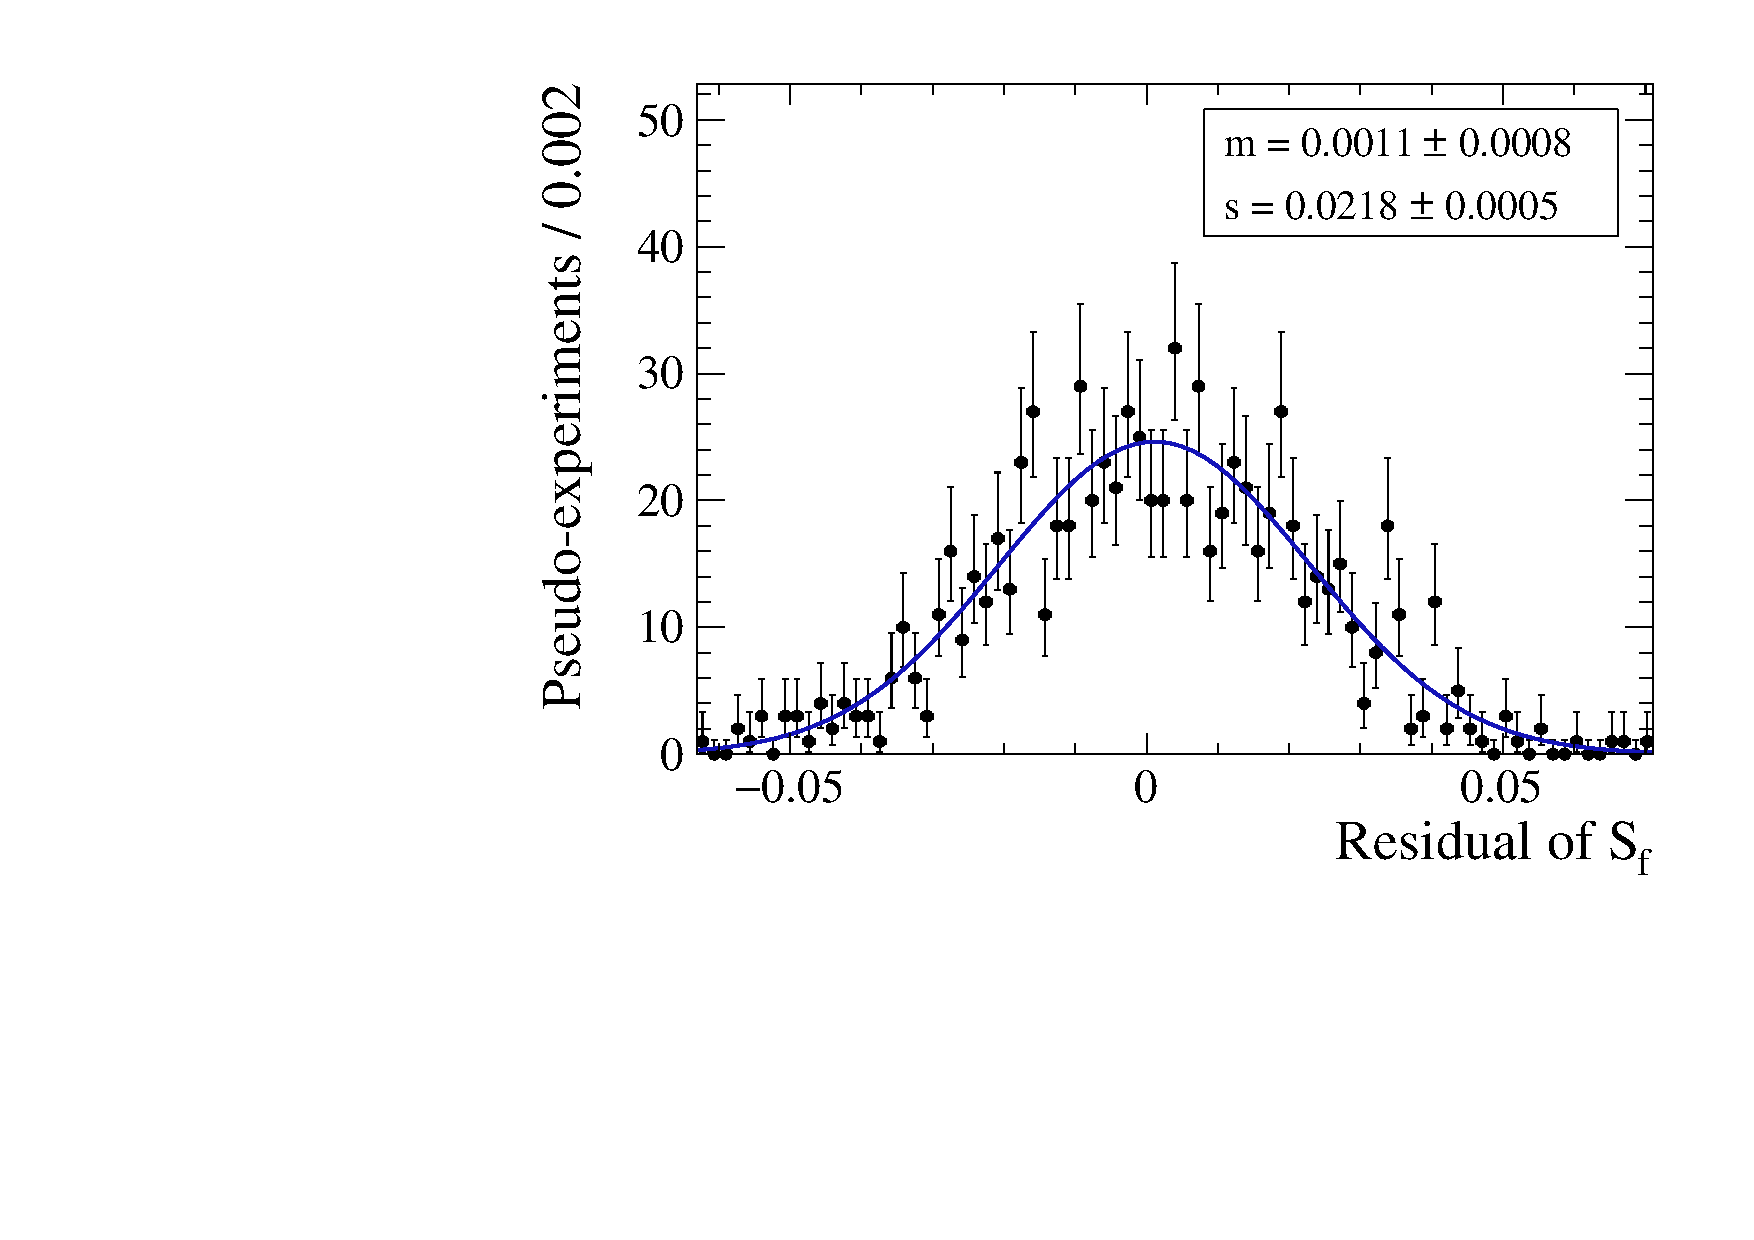
\includegraphics[width=0.4\textwidth]{06Systematics/figs/FT_Sf_res.pdf}
		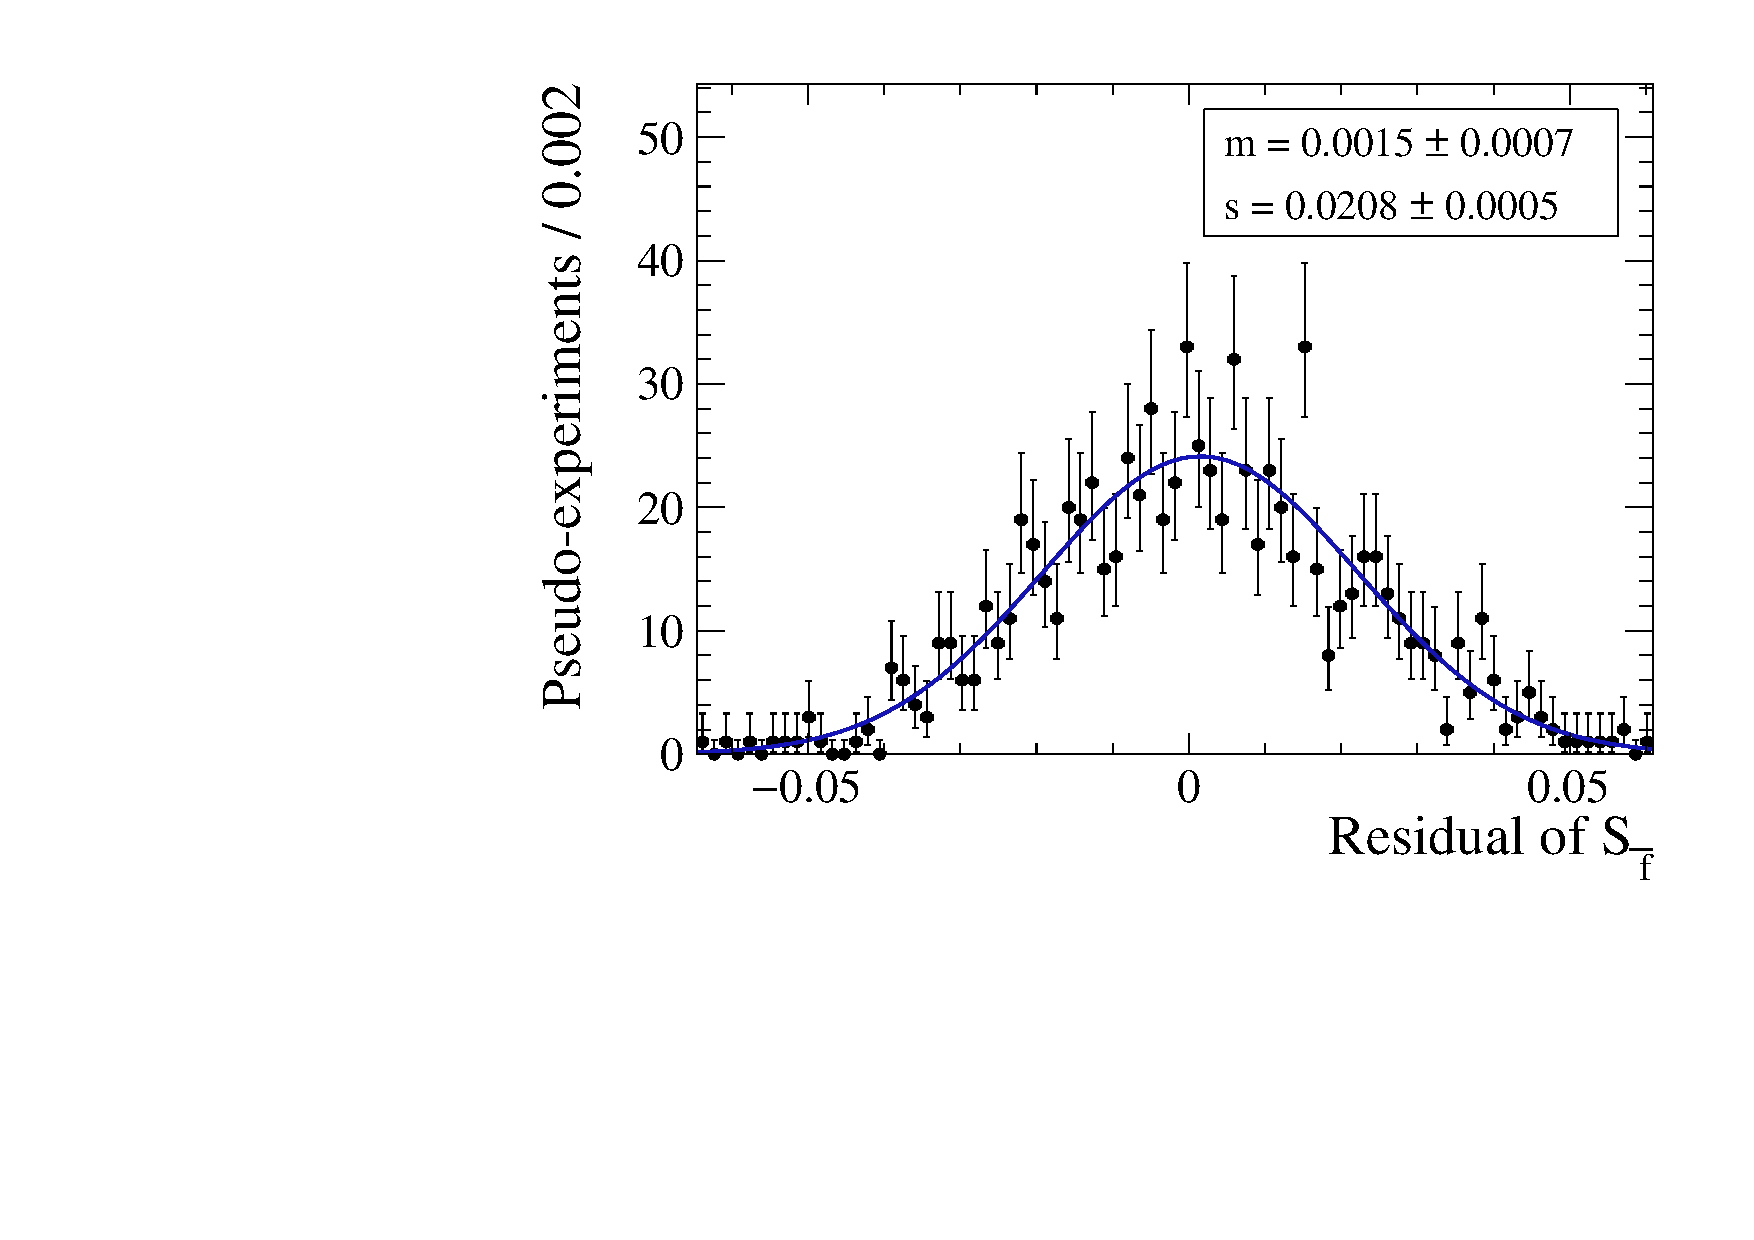
\includegraphics[width=0.4\textwidth]{06Systematics/figs/FT_Sfbar_res.pdf}
	\end{center}
        \vspace{-2mm}
	\caption{Distribution of $S_f$ (left) and $S_{\bar f}$ (right) residuals for the determination of the systematic uncertainty due to the tagging calibration
	models.}
	\label{fig:FTSystToys}
\end{figure}

%-------------------------------------------------------------------------------
\subsubsection{Flavour tagging efficiency asymmetries}
\label{sec:syst_toys_tageffAsym}

Toys are generated with the flavour tagging asymmetries set to their (negative) estimate from simulation minus their
uncertainty, namely \SI{-0.14}{\percent} and \SI{-0.13}{\percent} for the OS and SS tagger, respectively.
The distributions of the residuals of \Sf~and \Sfb~are shown in Fig.~\ref{fig:FTEffAsym}. The residuals are not compatible with
zero and therefore they are assigned as systematic uncertainties.
\begin{figure}[t]
	\begin{center}
		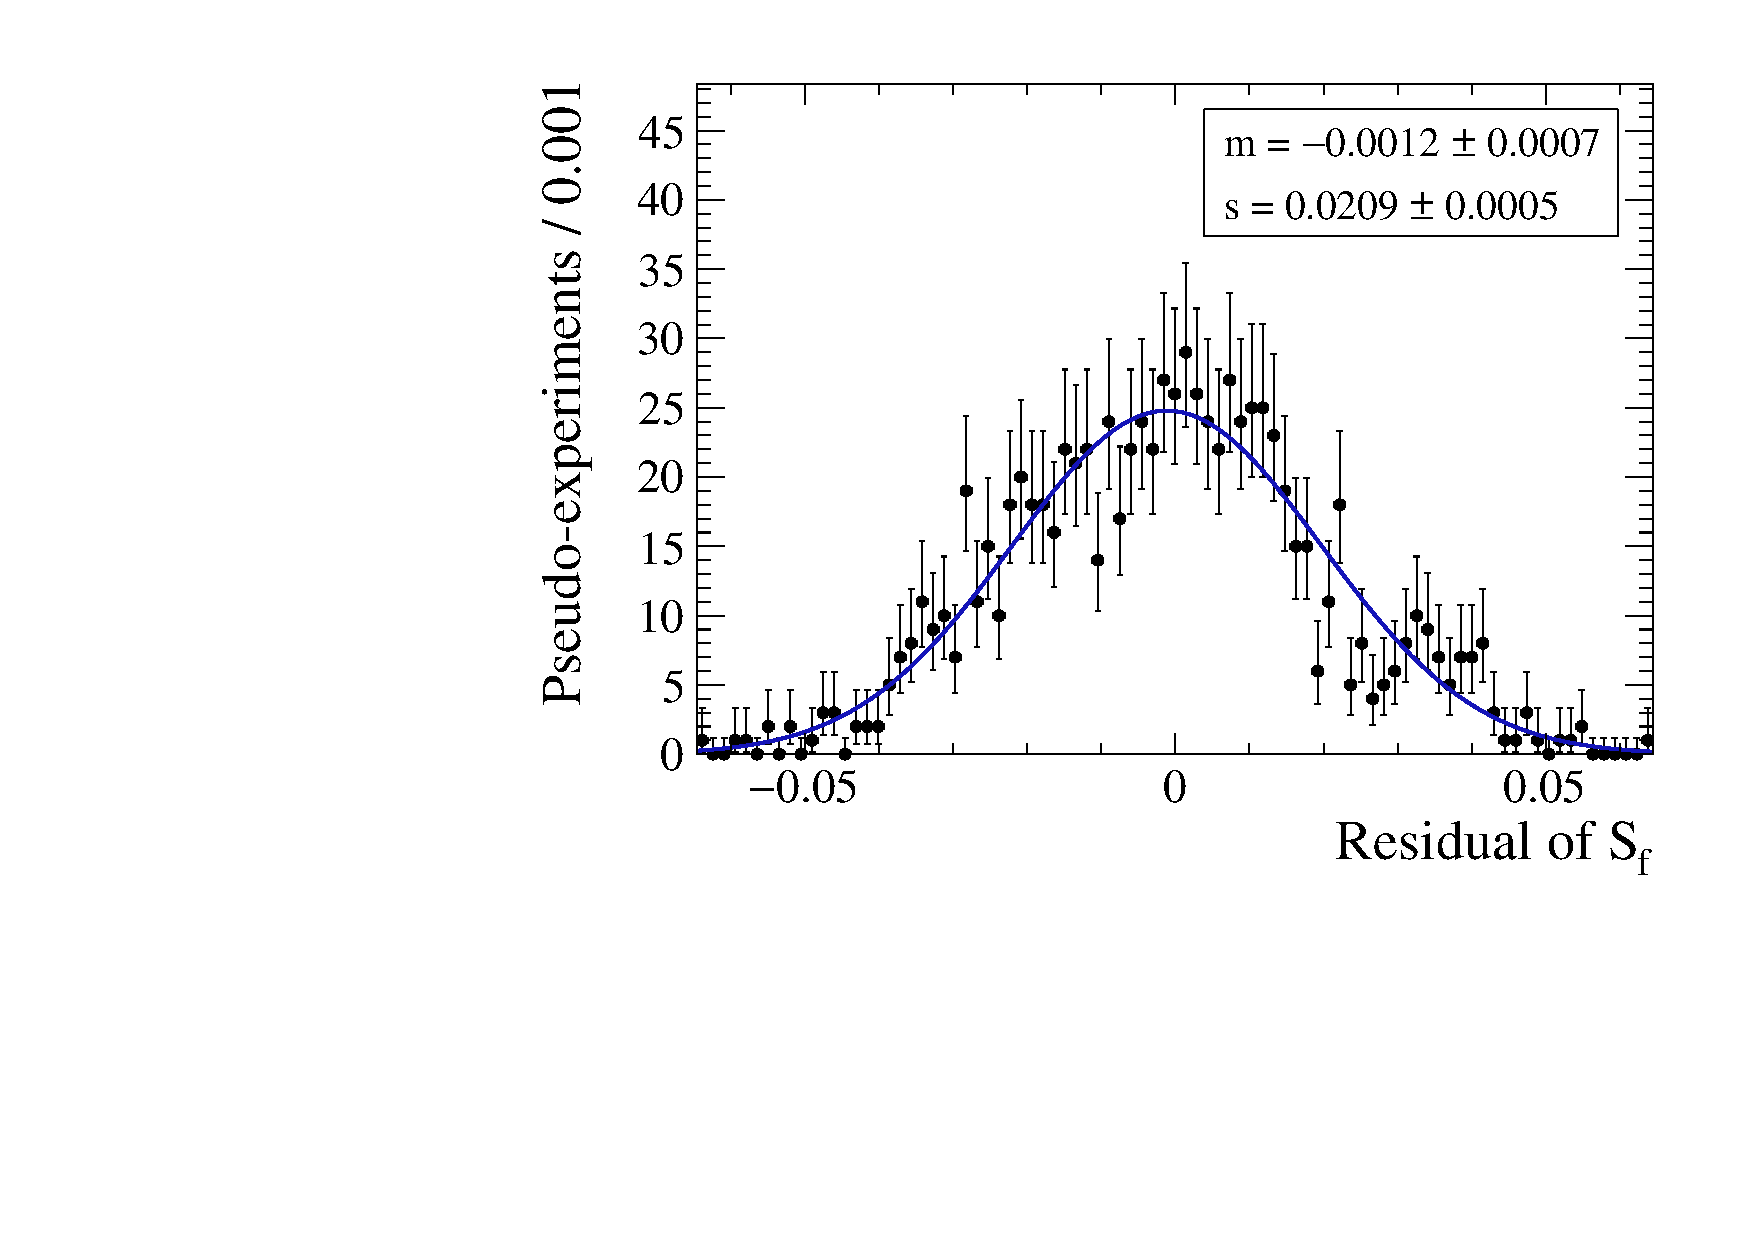
\includegraphics[width=0.4\textwidth]{06Systematics/figs/FTeffAsym_Sf_res.pdf}
		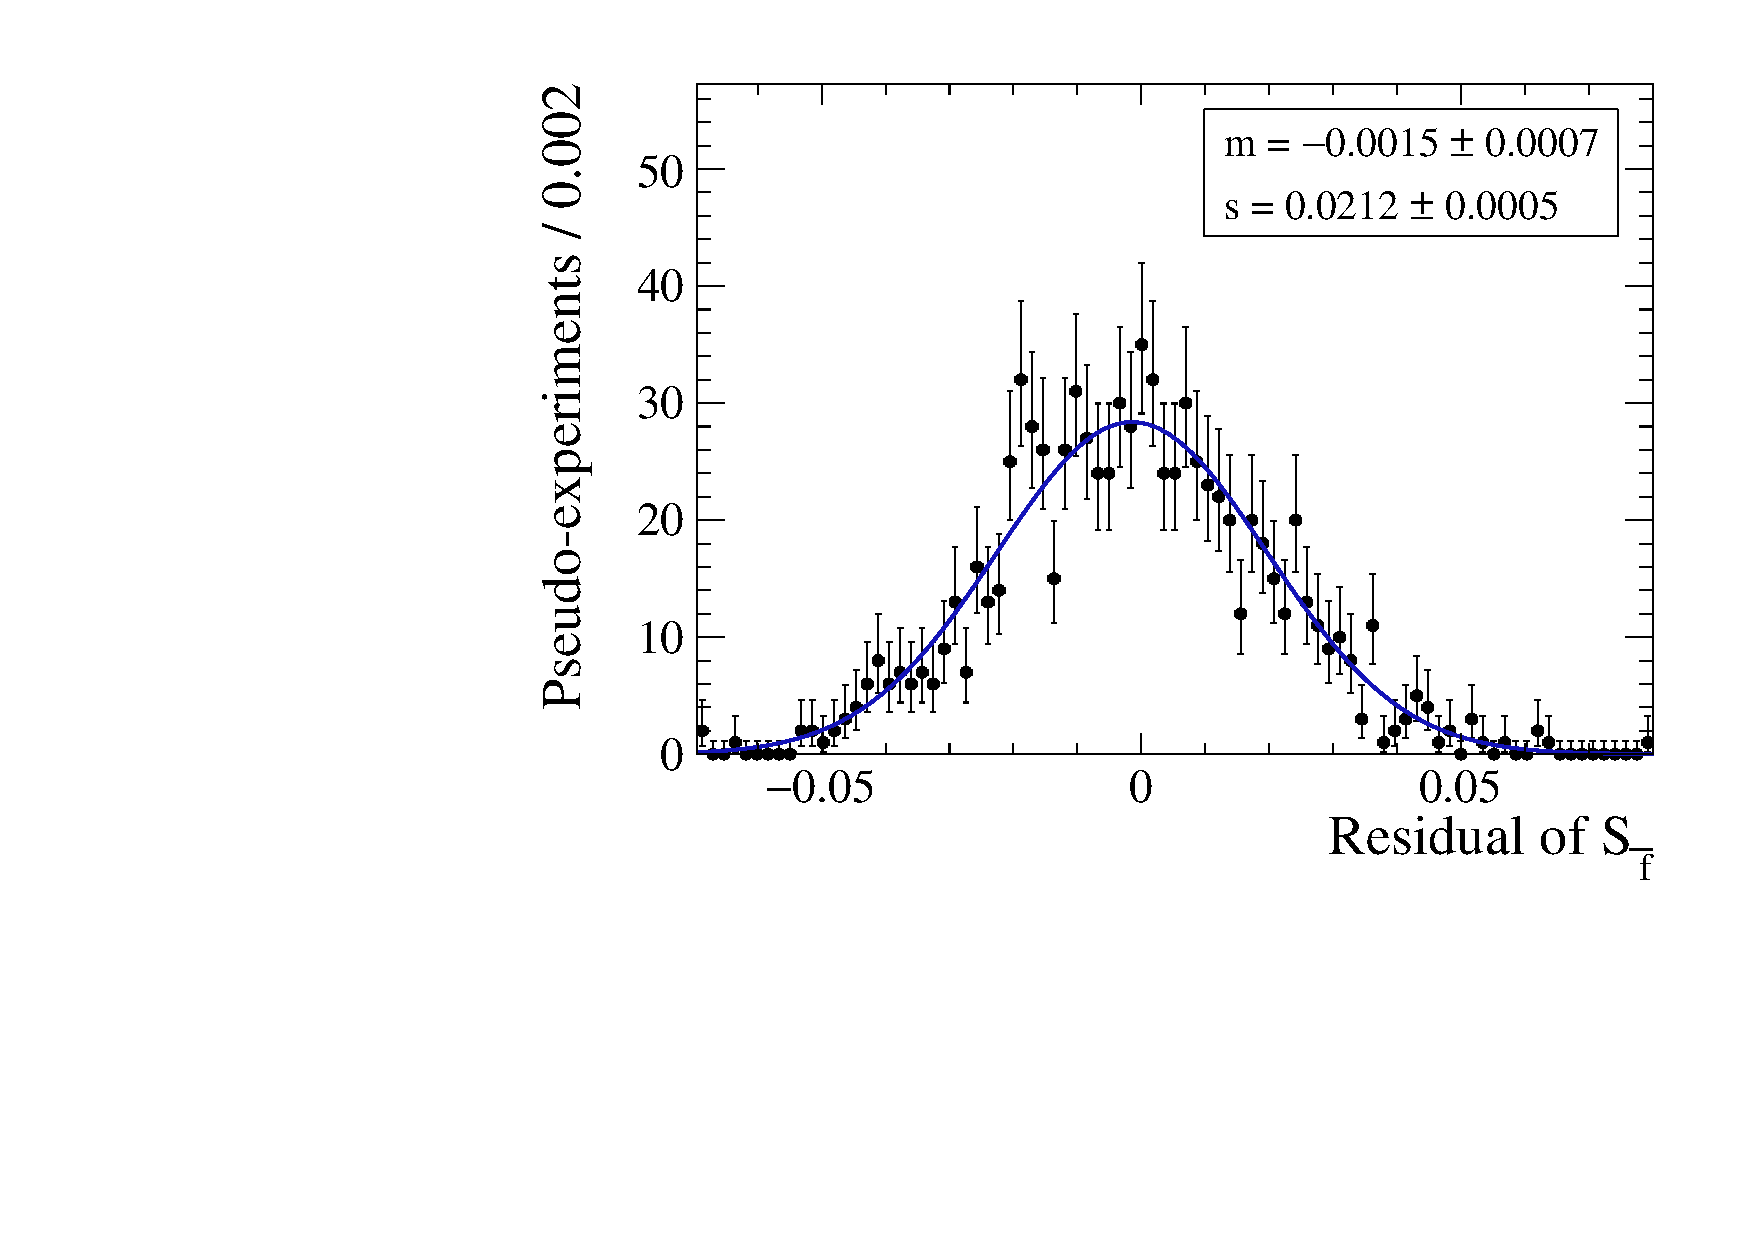
\includegraphics[width=0.4\textwidth]{06Systematics/figs/FTeffAsym_Sfbar_res.pdf}
	\end{center}
        \vspace{-2mm}
	\caption{Distribution of $S_f$ (left) and $S_{\bar f}$ (right) residuals for the determination of the systematic uncertainty due to the assumption on
	the flavour tagging efficiency asymmetry.}
	\label{fig:FTEffAsym}
\end{figure}

%-------------------------------------------------------------------------------
\subsubsection{Acceptance model}
\label{sec:syst_toys_acceptancemodel}

The acceptance model is modified in the generation by replacing the nominal knots for the spline function with new knots,
namely at 0.4, 0.45, 0.8, 1.3, 2.5, 6.0, and 12.0 ps. The distribution of the residuals of
\Sf~and \Sfb~are shown in Fig.~\ref{fig:acceptanceSystToys}. Residuals consistent with zero are found
and therefore the uncertainty on the residuals is assigned as systematic uncertainty.
\begin{figure}[t]
	\begin{center}
		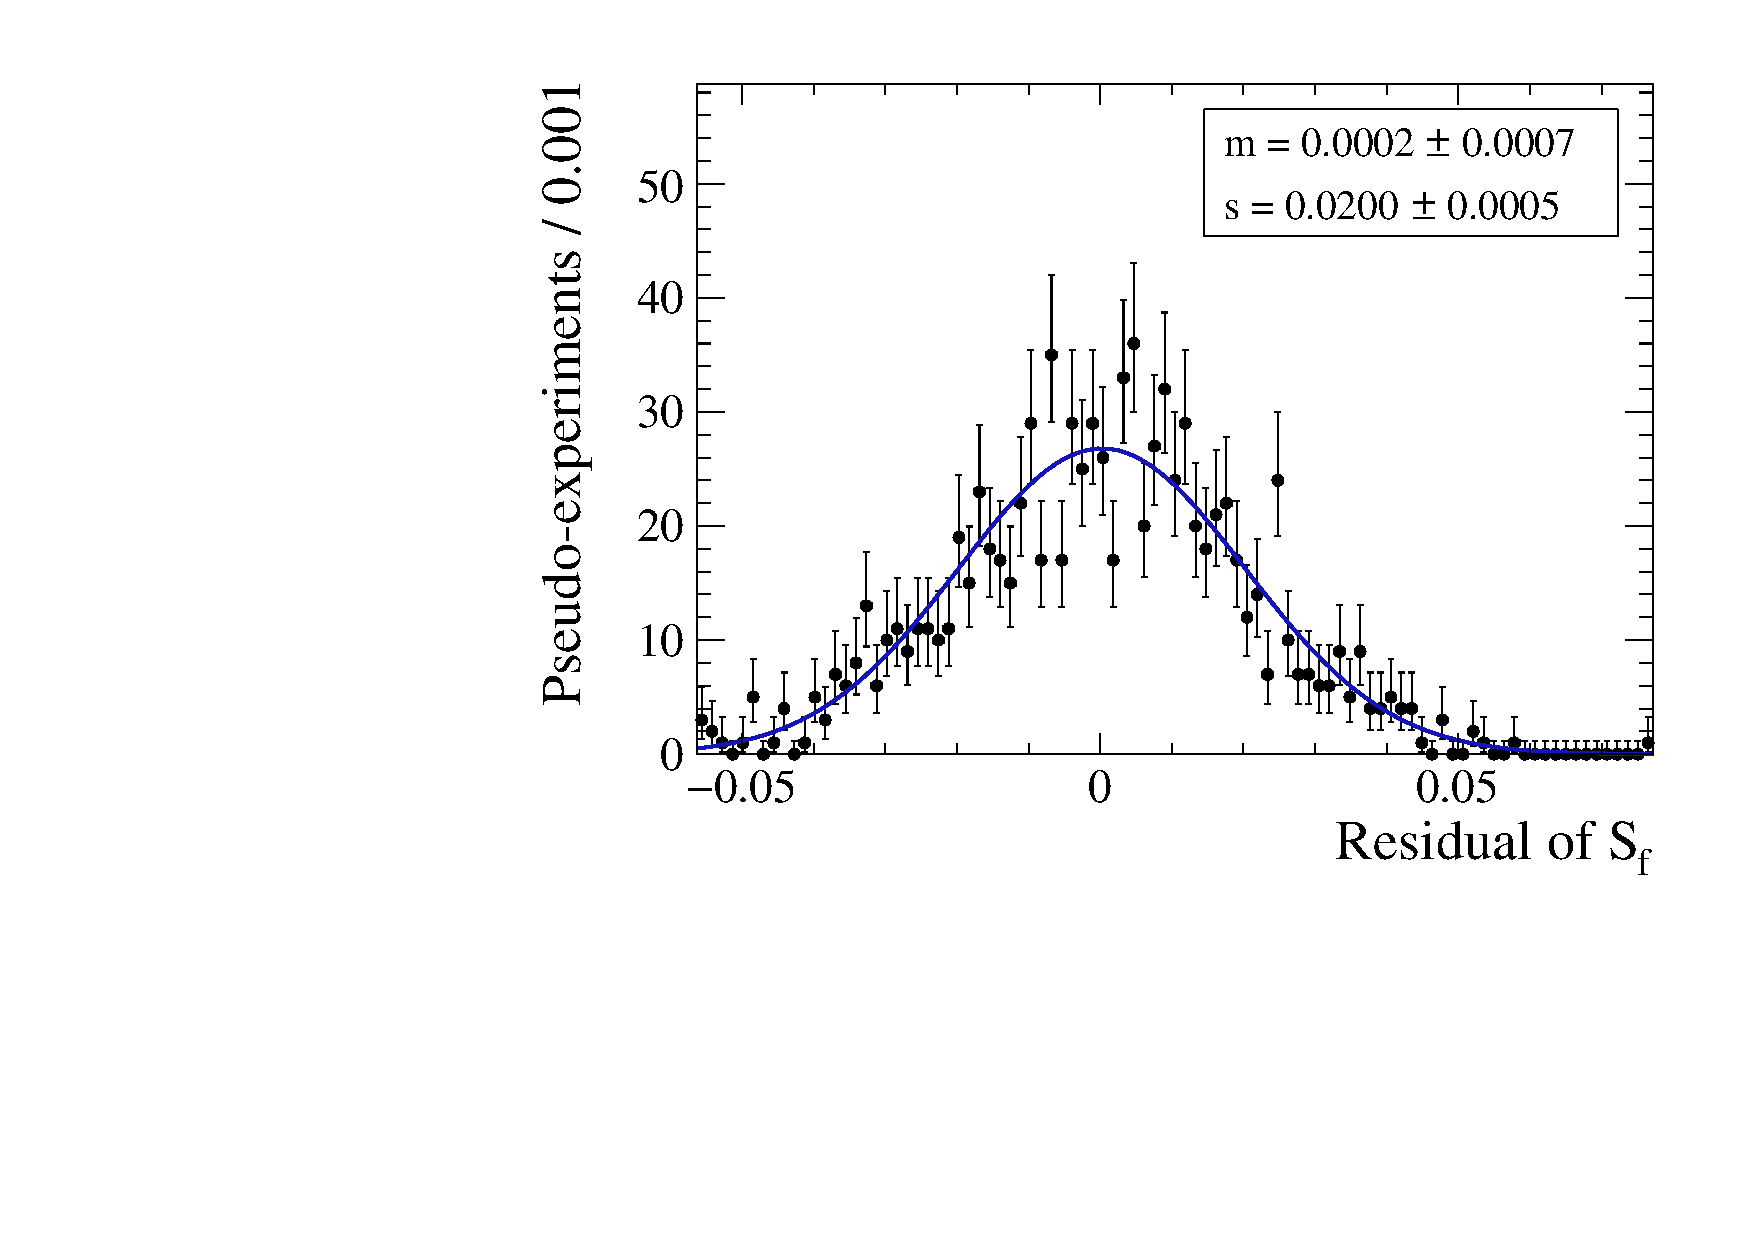
\includegraphics[width=0.4\textwidth]{06Systematics/figs/accept_Sf_res.pdf}
		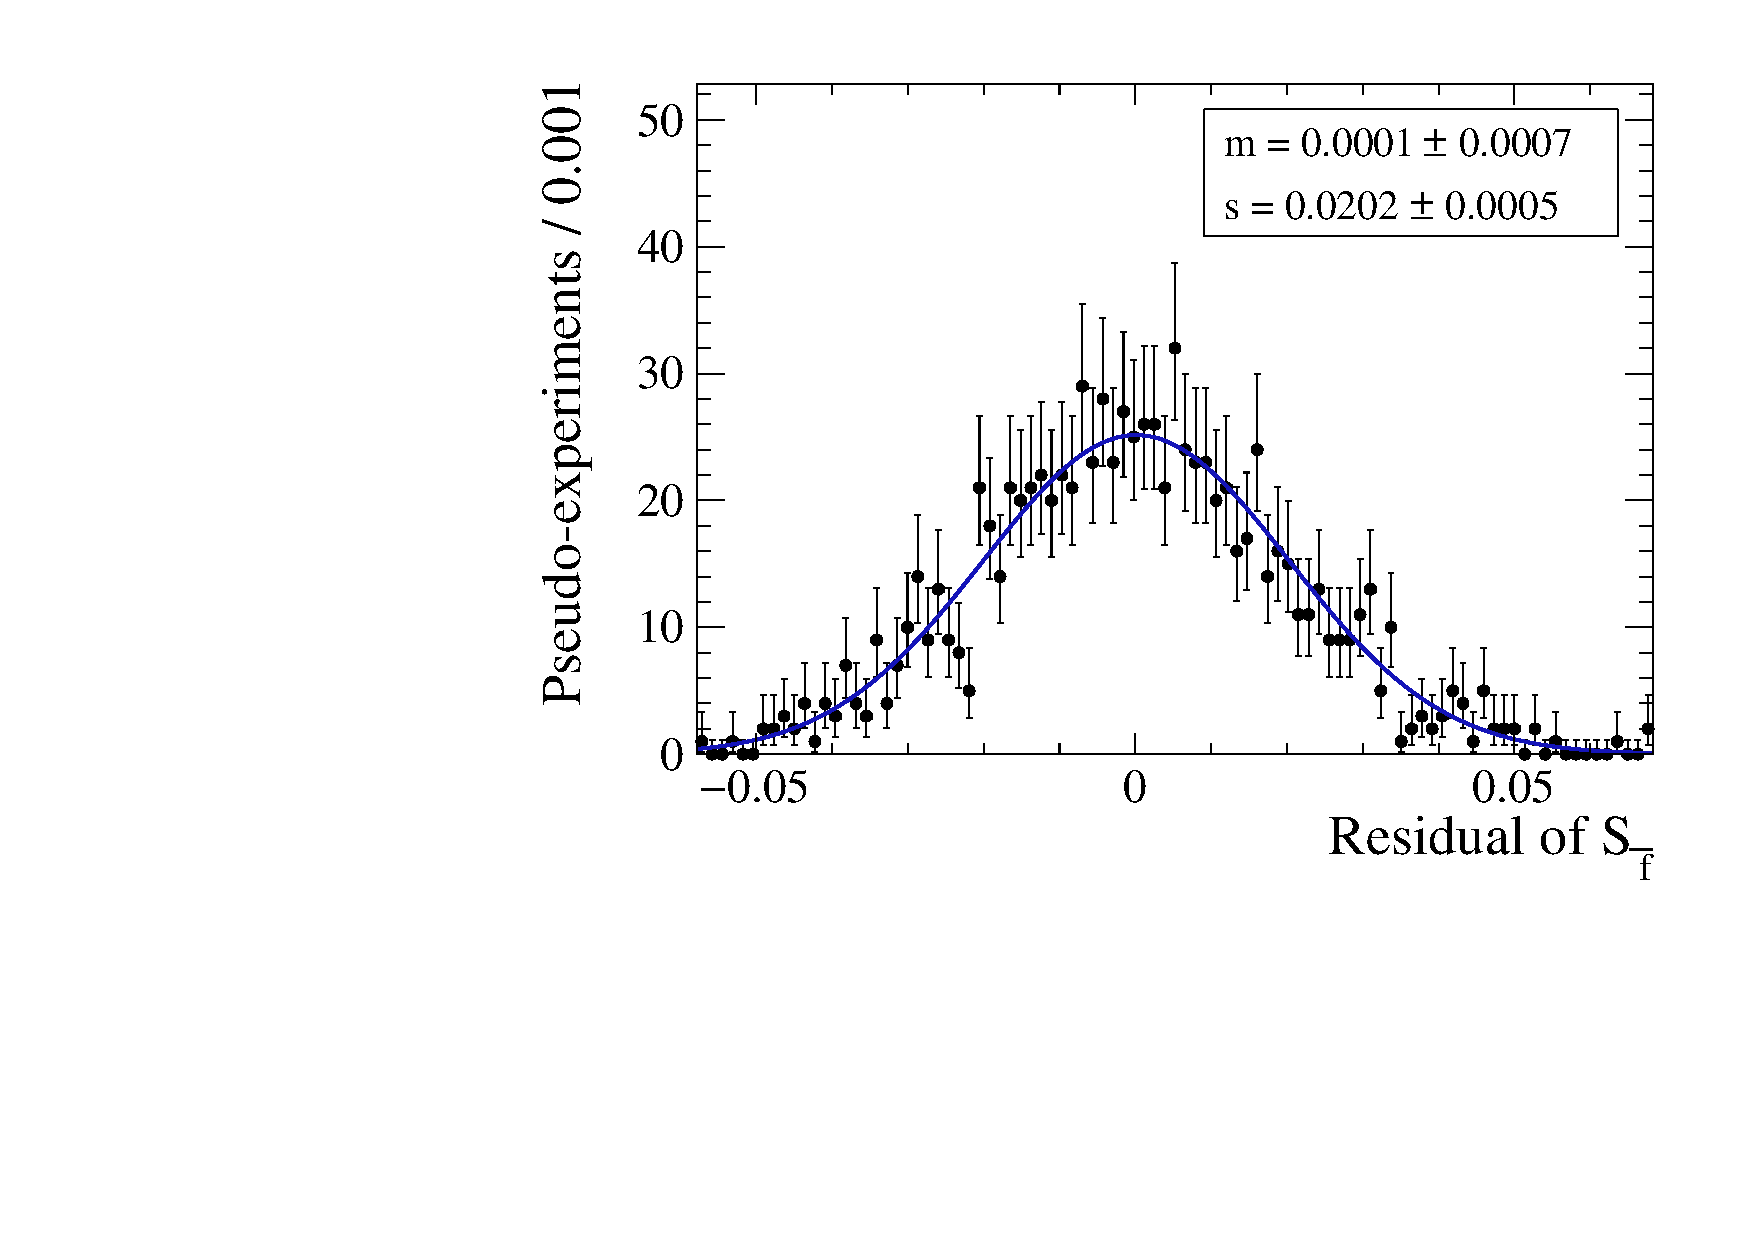
\includegraphics[width=0.4\textwidth]{06Systematics/figs/accept_Sfbar_res.pdf}
	\end{center}
        \vspace{-2mm}
	\caption{Distribution of $S_f$ (left) and $S_{\bar f}$ (right) residuals for the determination of the systematic uncertainty due to the acceptance model.}
	\label{fig:acceptanceSystToys}
\end{figure}

\subsubsection{Decay time resolution}
\label{sec:syst_toys_resolution}
Toys are generated with time resolutions $20\fs$ larger and $20\fs$ smaller than the nominal value of 55\fs.
The distributions of the fitted value of \Sf~and \Sfb~are shown in Fig.~\ref{fig:ToysAllFixedCPloRes}.
The largest residual is considered as overall systematic uncertainty.
\begin{figure}[t]
        \begin{center}
                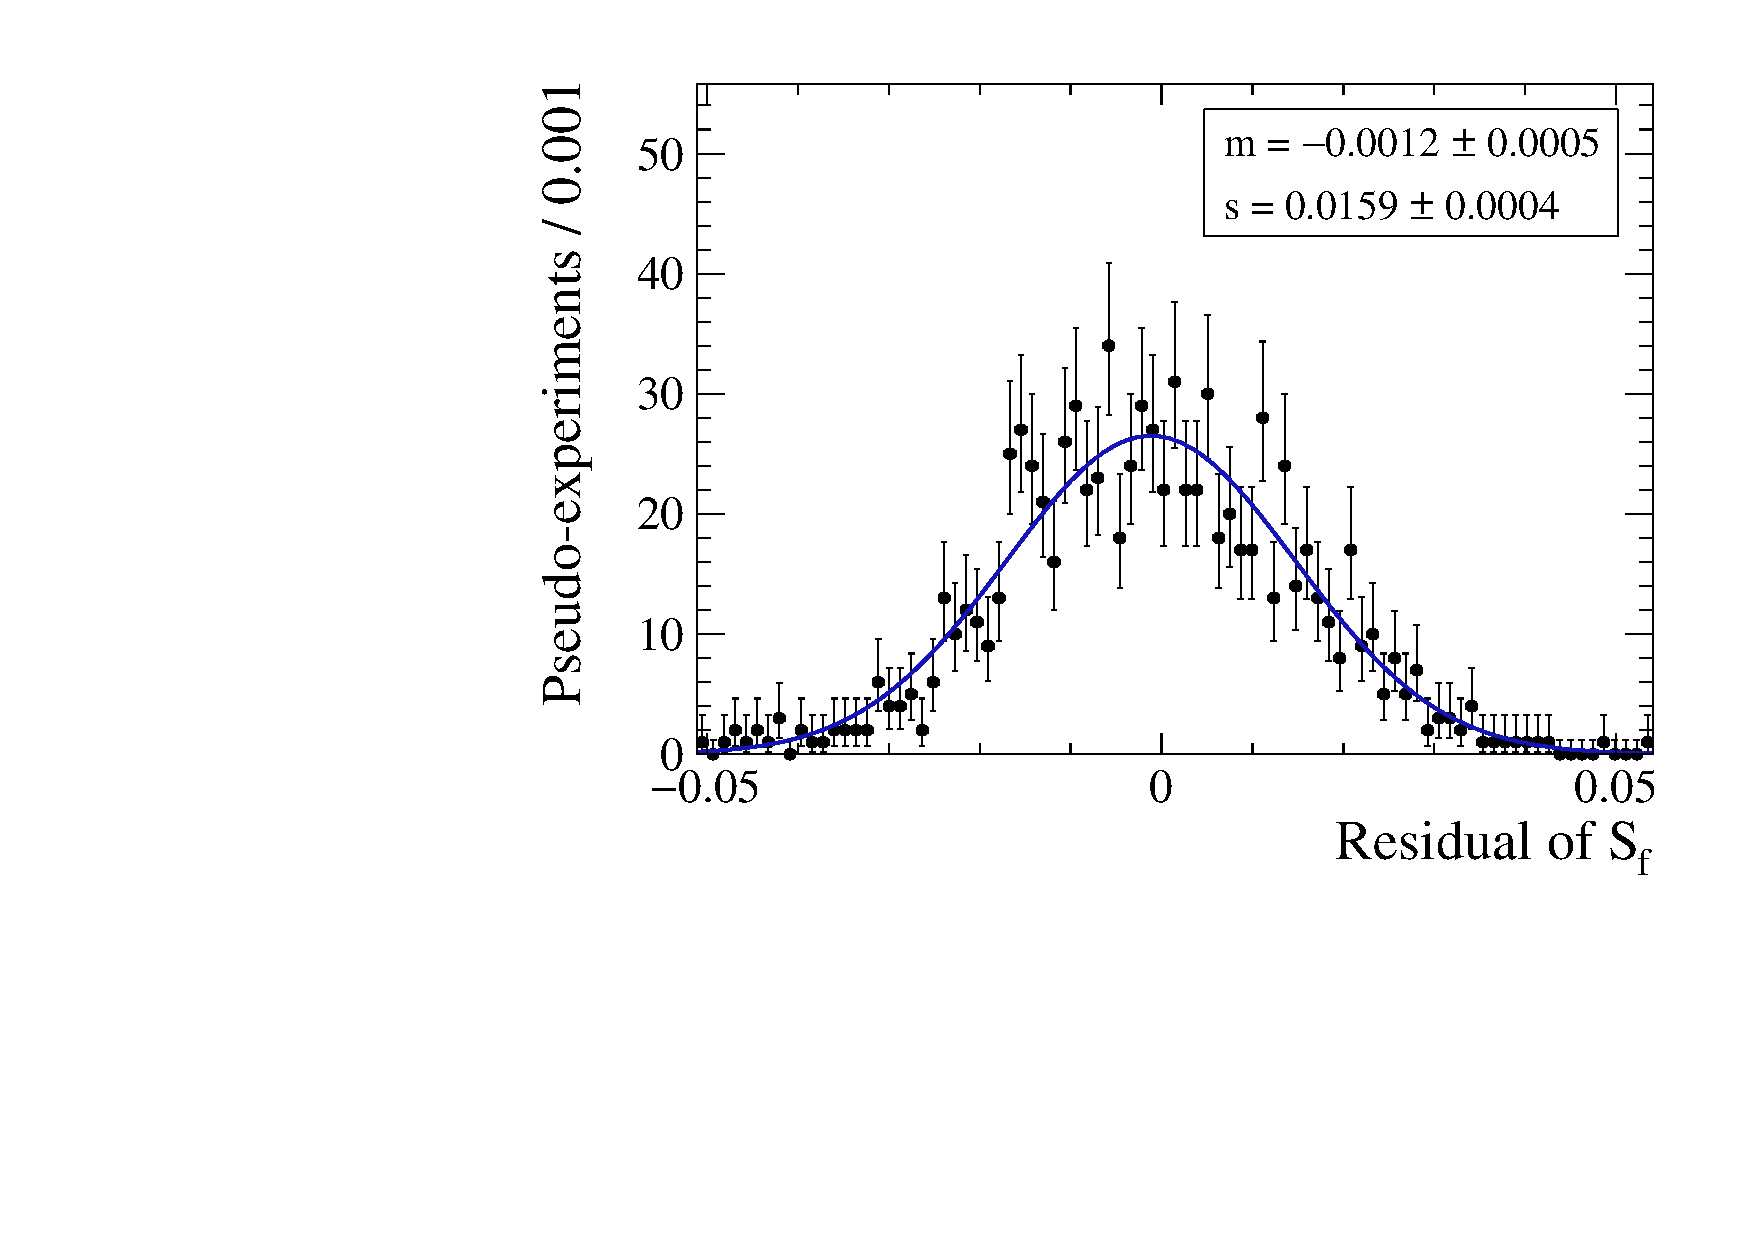
\includegraphics[width=0.4\linewidth]{06Systematics/figs/ResHigh_Sf_res.pdf}
                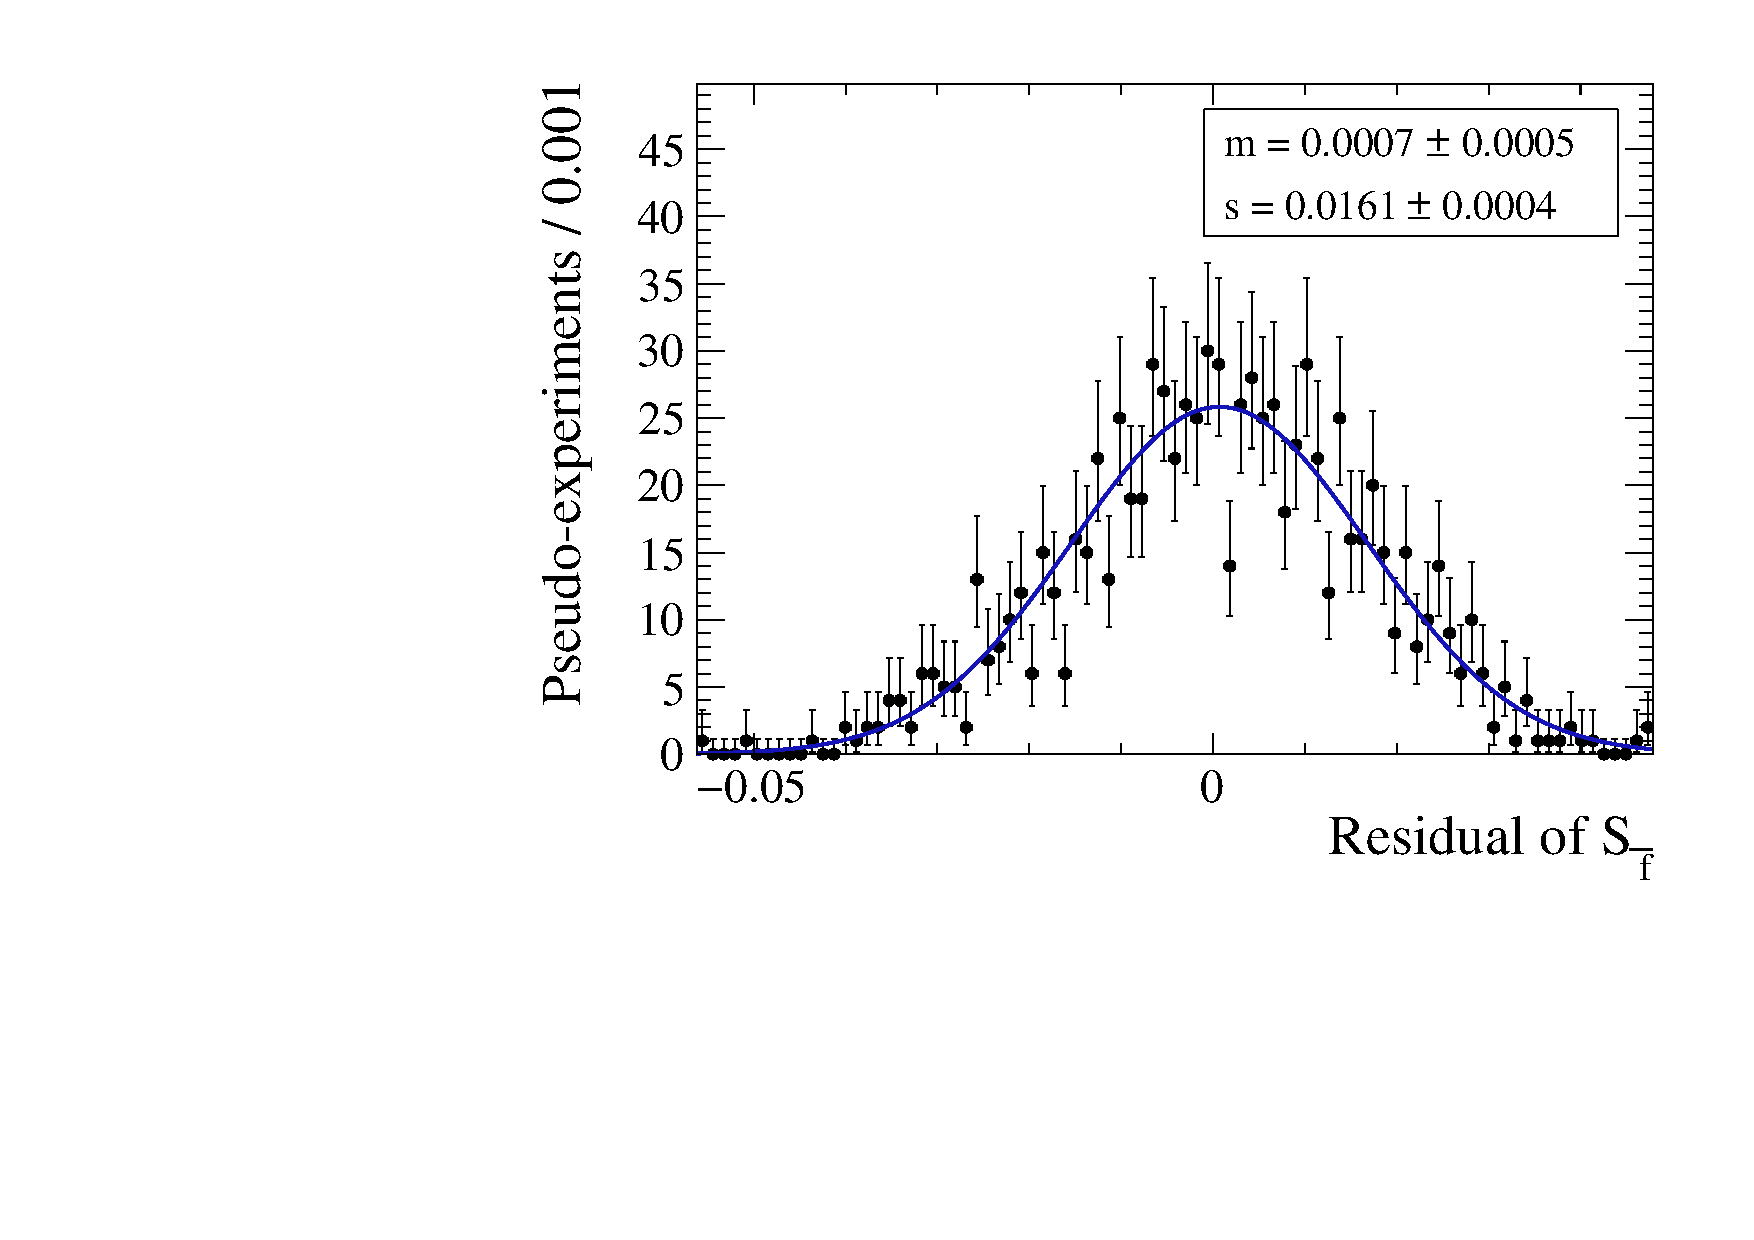
\includegraphics[width=0.4\linewidth]{06Systematics/figs/ResHigh_Sfbar_res.pdf} \\
                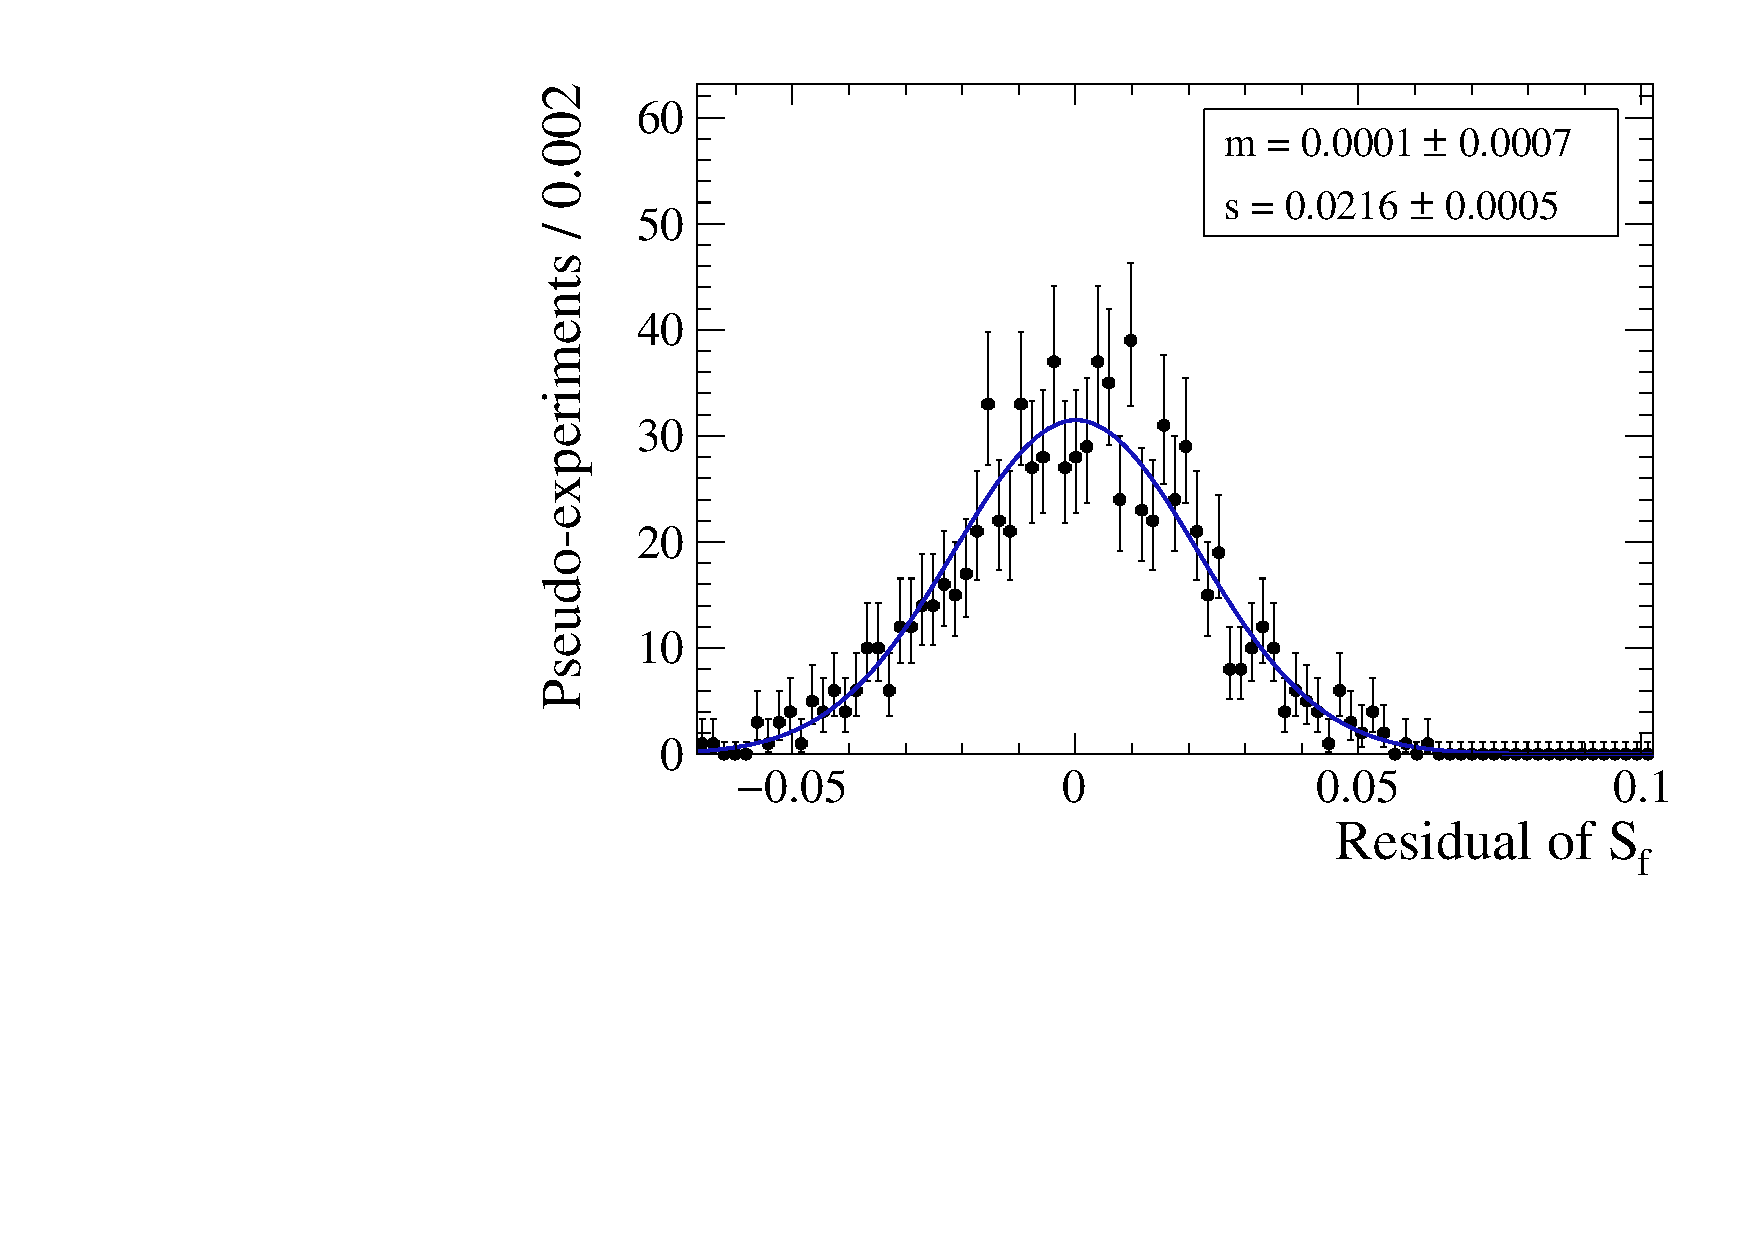
\includegraphics[width=0.4\linewidth]{06Systematics/figs/ResLow_Sf_res.pdf}
                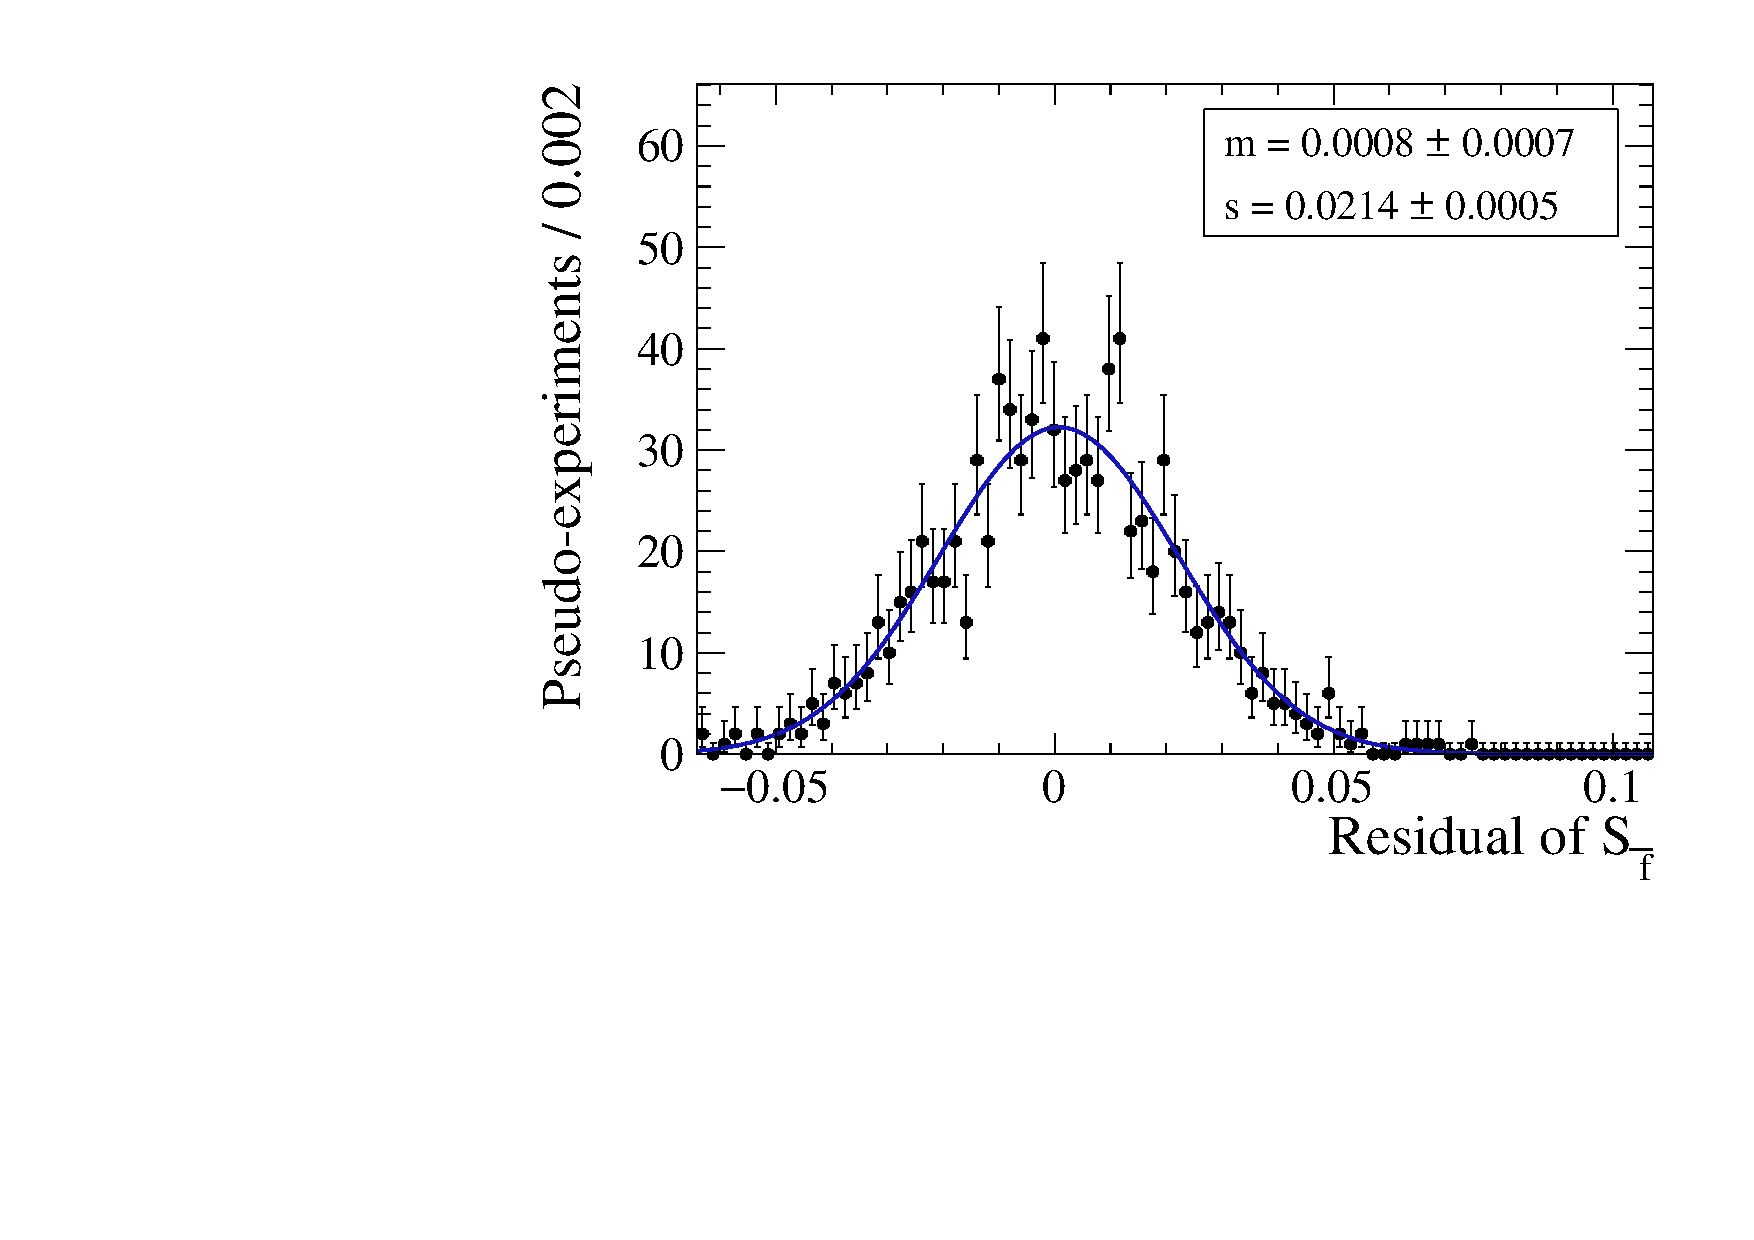
\includegraphics[width=0.4\linewidth]{06Systematics/figs/ResLow_Sfbar_res.pdf}
                \end{center}
        \vspace{-2mm}
        \caption{Distribution of $S_f$ (left) and $S_{\bar f}$ (right) residuals for the determination of the systematic uncertainty due
        to the resolution model. Top: \SI{75}{\fs} resolution model. Bottom: \SI{35}{\fs} resolution
        model. }
        \label{fig:ToysAllFixedCPloRes}
\end{figure}

%-------------------------------------------------------------------------------
\subsubsection[Fixed $C_f$]{Fixed \boldmath{$C_f$}}
\label{sec:syst_toys_fixC}

Toys are generated with $C_f=-C_{\bar f}$ set to the average of the measurements by \belle~and \babar~minus the
largest uncertainty among the two measurements, namely $0.993$~\cite{Aubert:2008zi, Das:2010be}.
The distributions of the residuals of \Sf~and \Sfb~are shown in Fig.~\ref{fig:CSystToys}. Residuals
consistent with zero are found, therefore the uncertainty on the residuals is assigned as systematic
uncertainty.
\begin{figure}[htbp]
	\begin{center}
		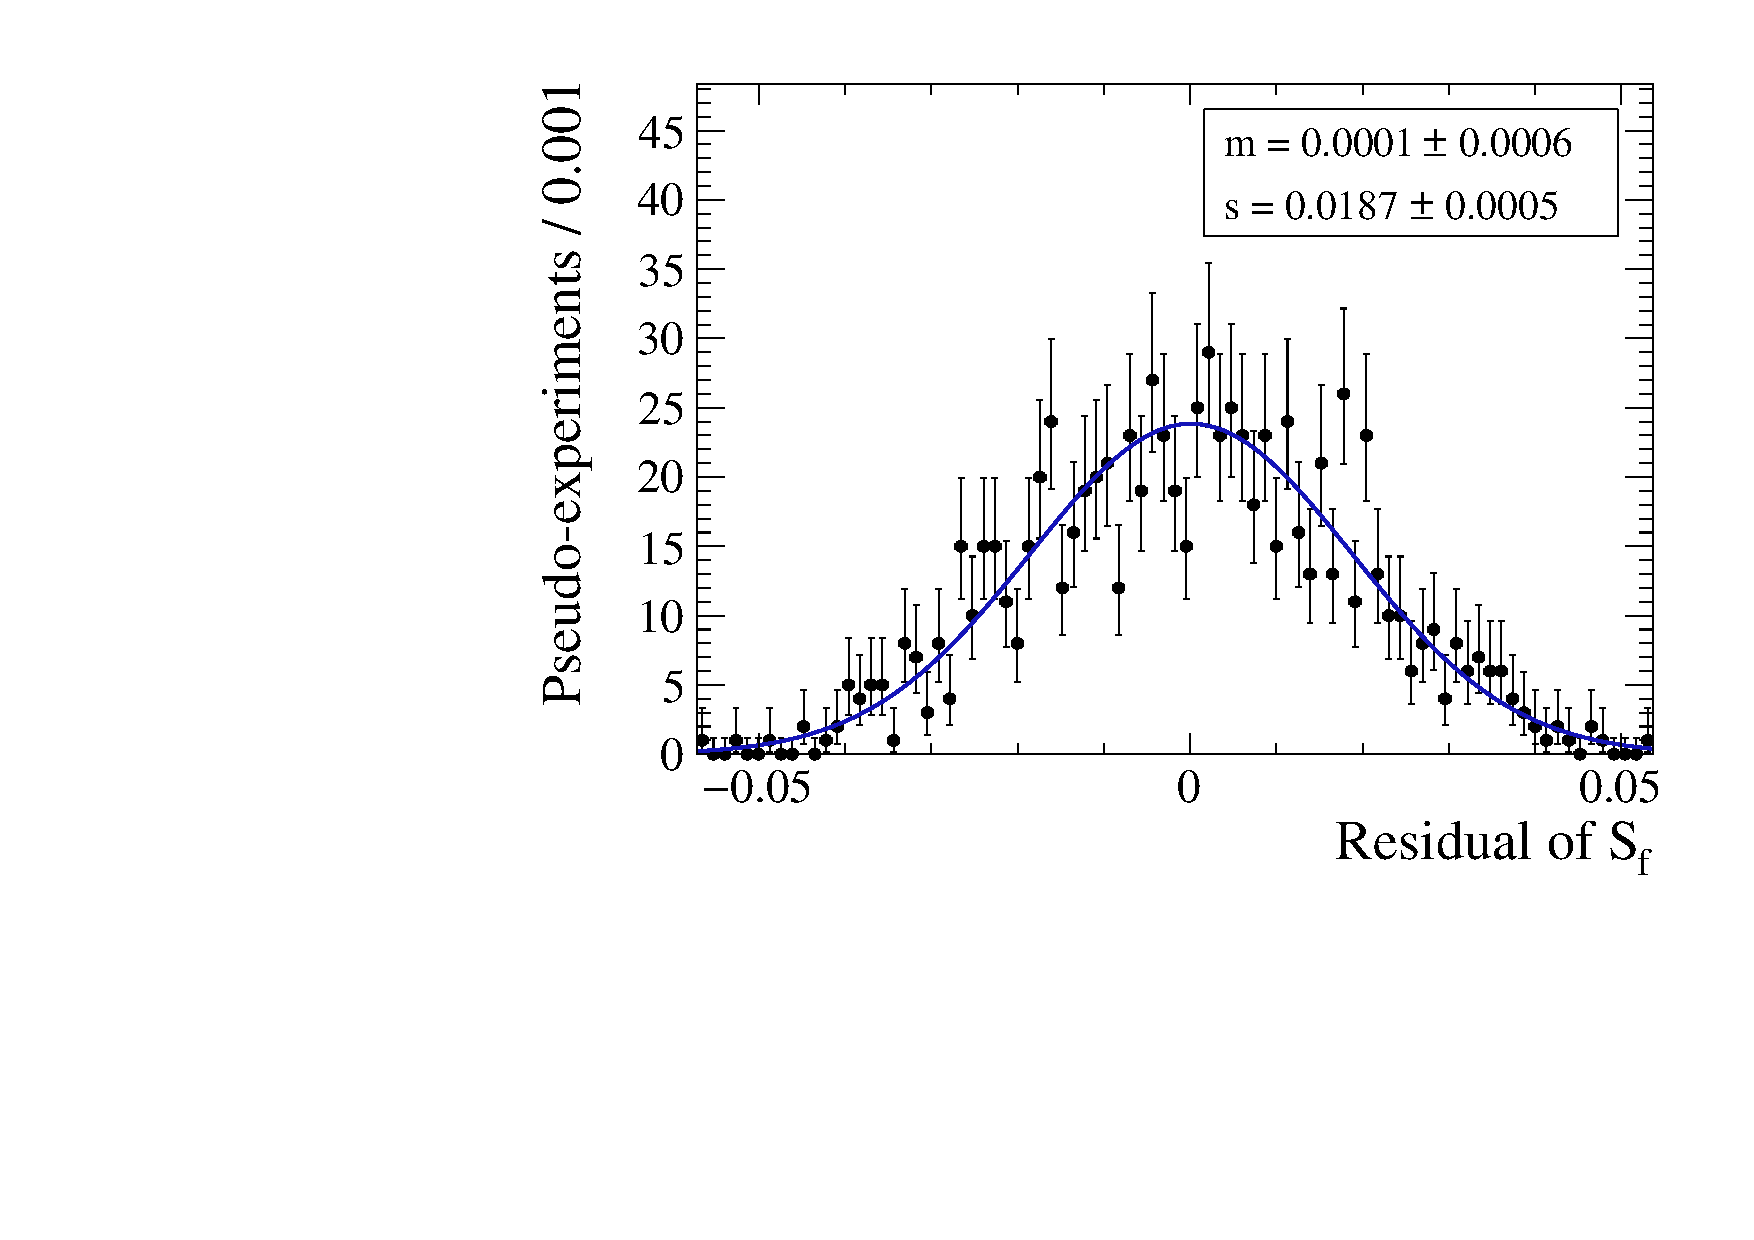
\includegraphics[width=0.4\textwidth]{06Systematics/figs/C_Sf_res.pdf}
		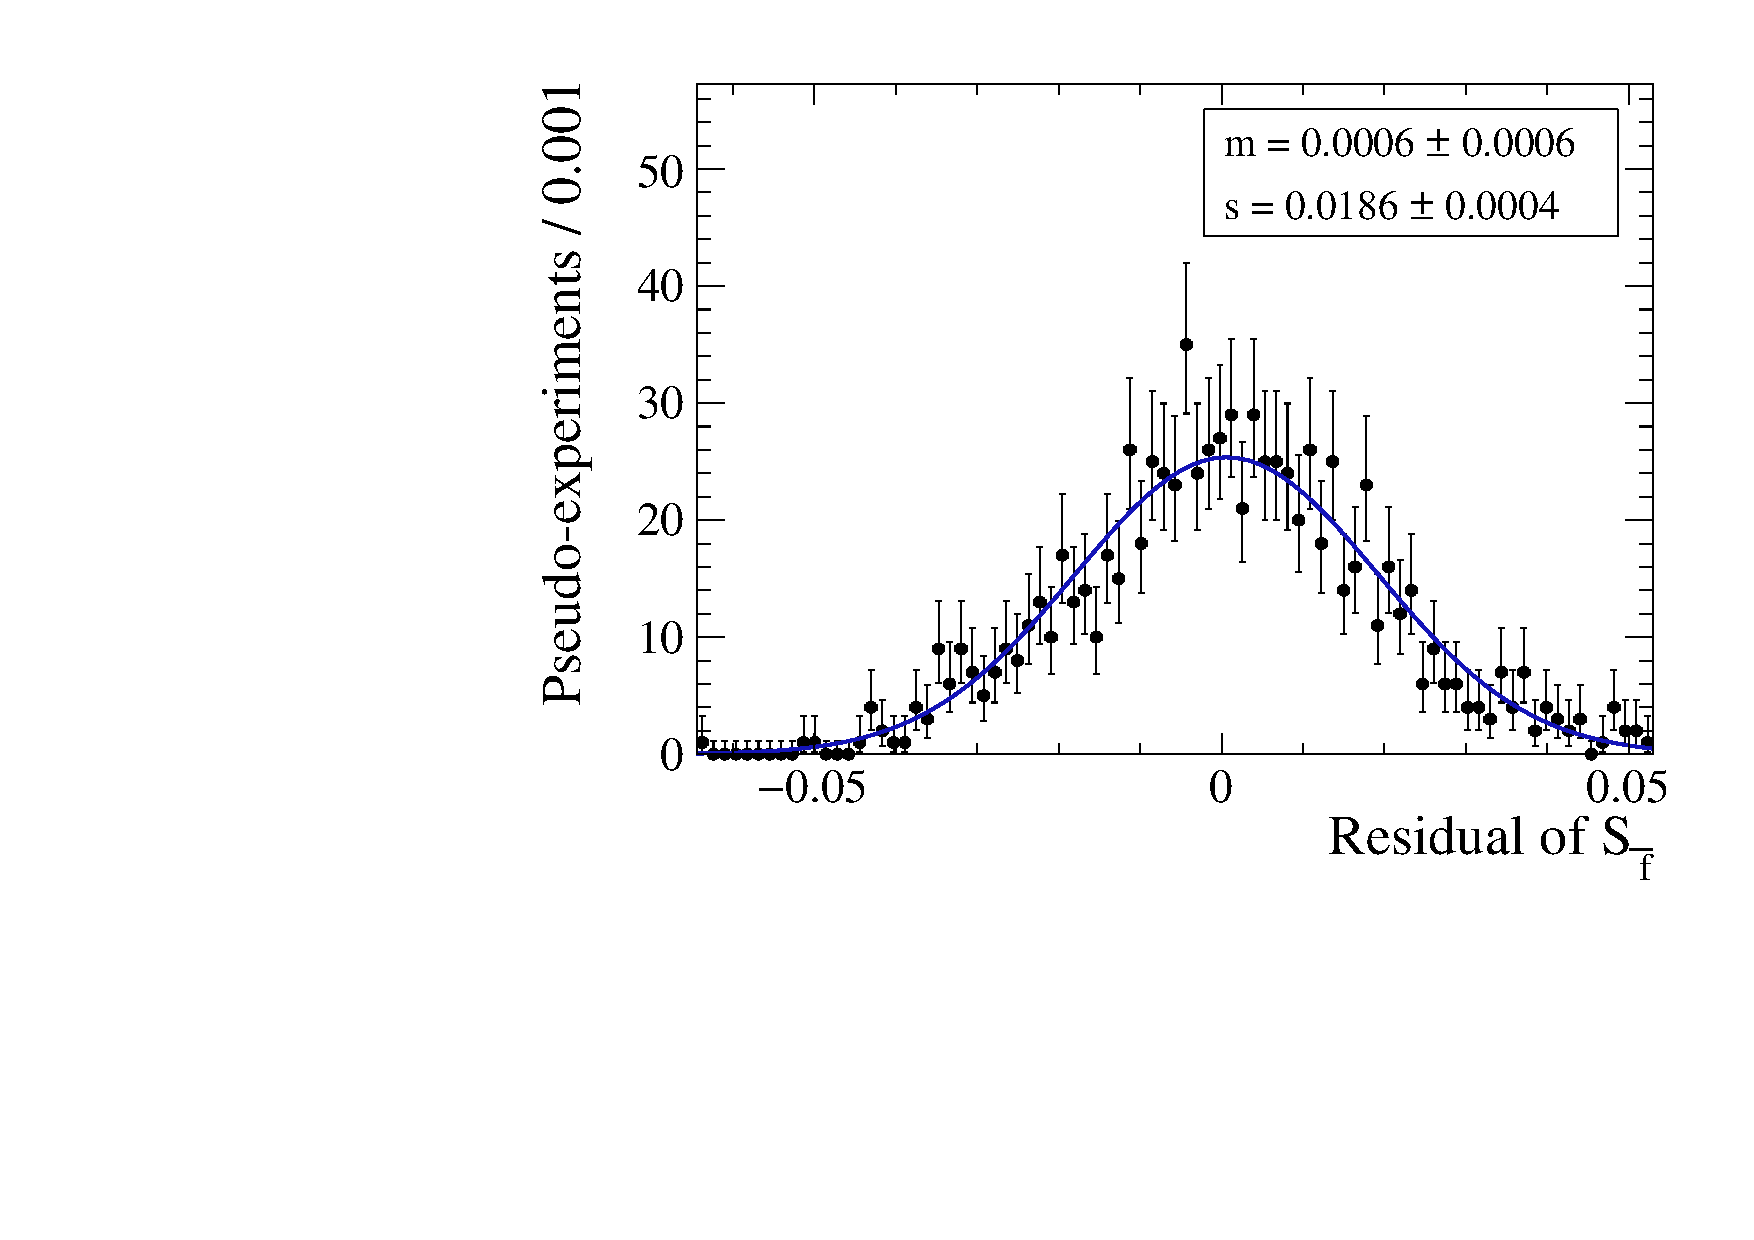
\includegraphics[width=0.4\textwidth]{06Systematics/figs/C_Sfbar_res.pdf}
	\end{center}
        \vspace{-2mm}
	\caption{Distribution of $S_f$ (left) and $S_{\bar f}$ (right) residuals for the determination of the systematic uncertainty due to the assumption $C_f=-C_{\bar f}=1$.}
	\label{fig:CSystToys}
\end{figure}

%-------------------------------------------------------------------------------
\subsubsection[Fixed $\Delta\Gamma$]{Fixed \boldmath{$\Delta\Gamma$}}
\label{sec:syst_toys_deltaGamma}

Toys are generated with \DG~set to the world average value plus its uncertainty, namely $0.0079\ps^{-1}$~\cite{HFAG}.
Moreover, the $D_{f}$ and $D_{\bar f}$ coefficients (defined in Eqs.~\ref{eq:P0tof}-\ref{eq:P0bartofbar}) have been fixed to their expected values of $-0.0103$ and $-0.0155$,
the same used in the Monte Carlo production of the $\Bz\to \Dm\pip$ sample (Appendix~\ref{app:mcgen}). The distribution of the residuals of \Sf~and
\Sfb~are shown in Fig.~\ref{fig:DGSystToys}. Residuals consistent with zero are found, therefore the uncertainty
on the residuals is assigned as systematic uncertainty.
\begin{figure}[t]
	\begin{center}
		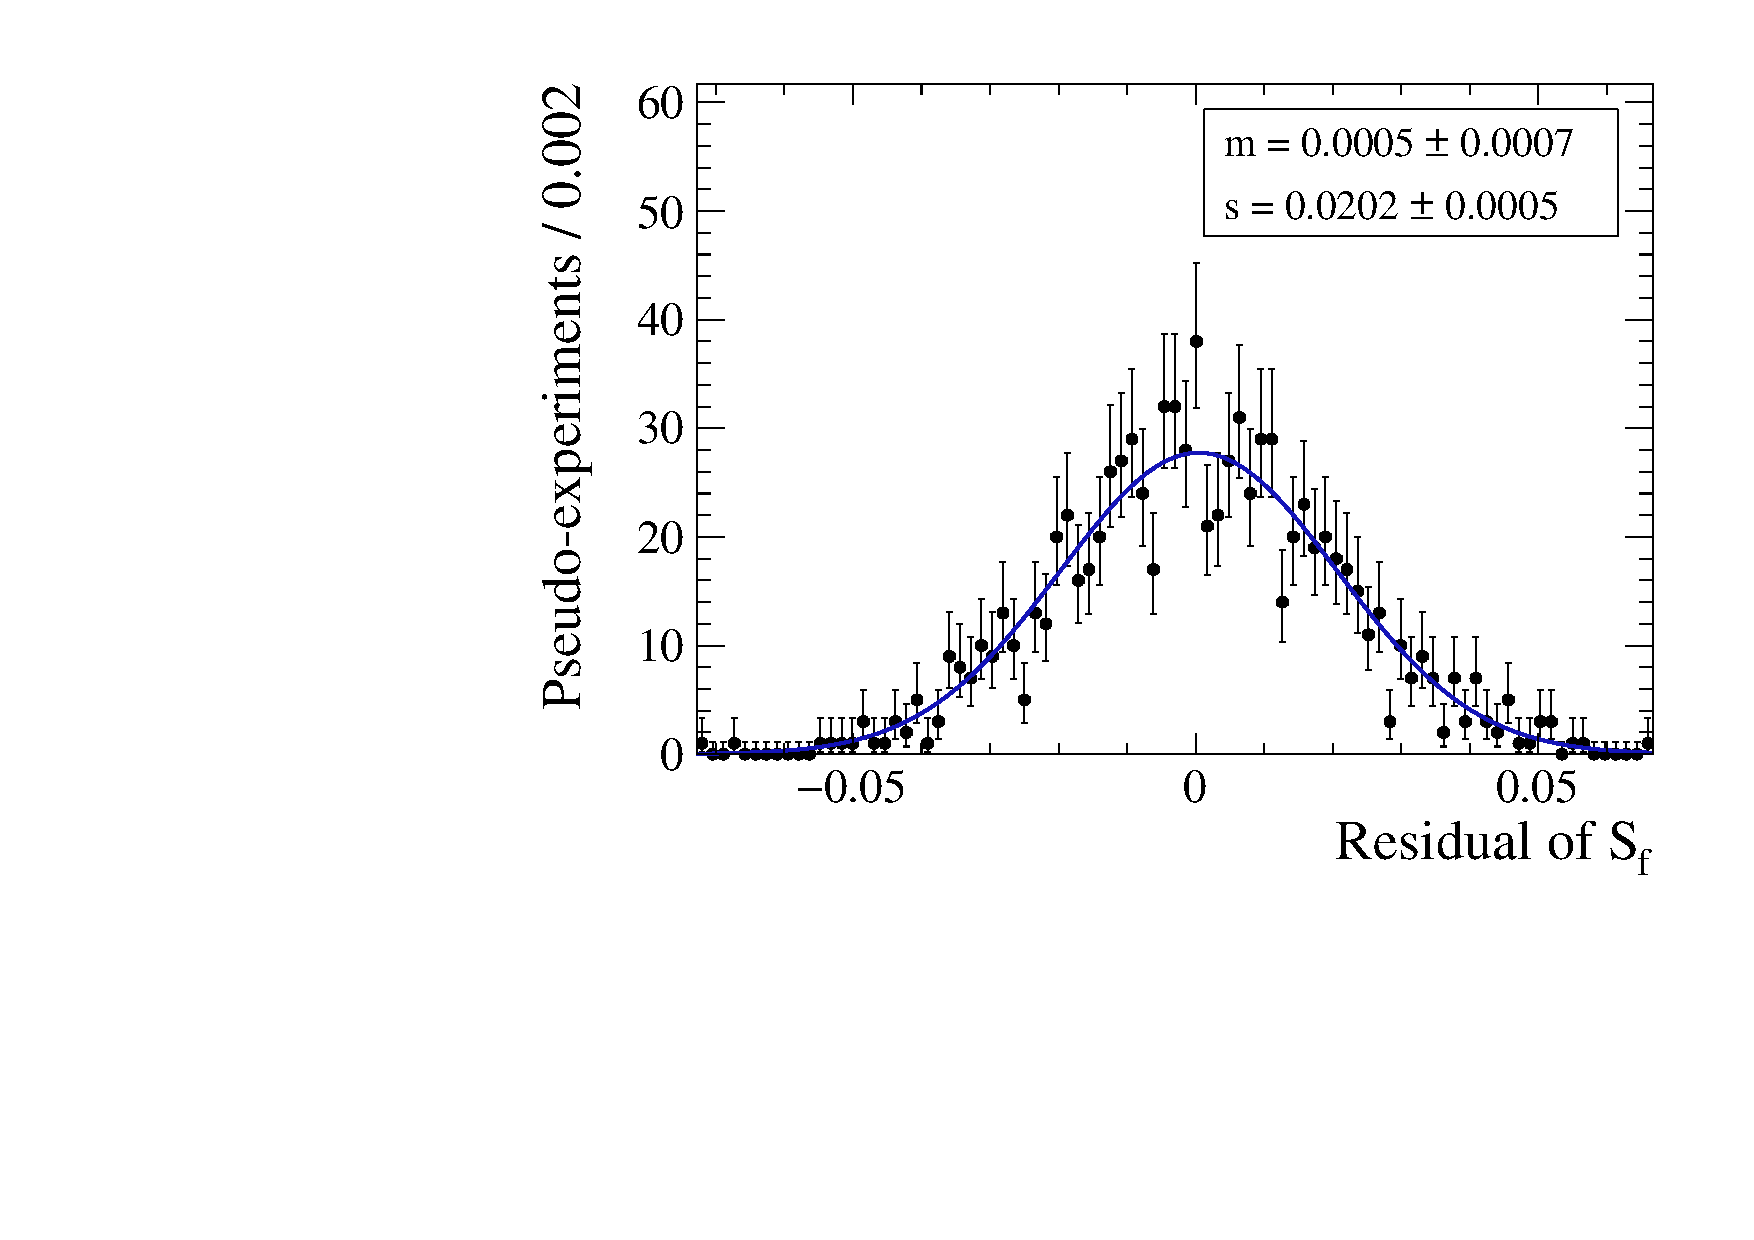
\includegraphics[width=0.4\textwidth]{06Systematics/figs/DG_Sf_res.pdf}
		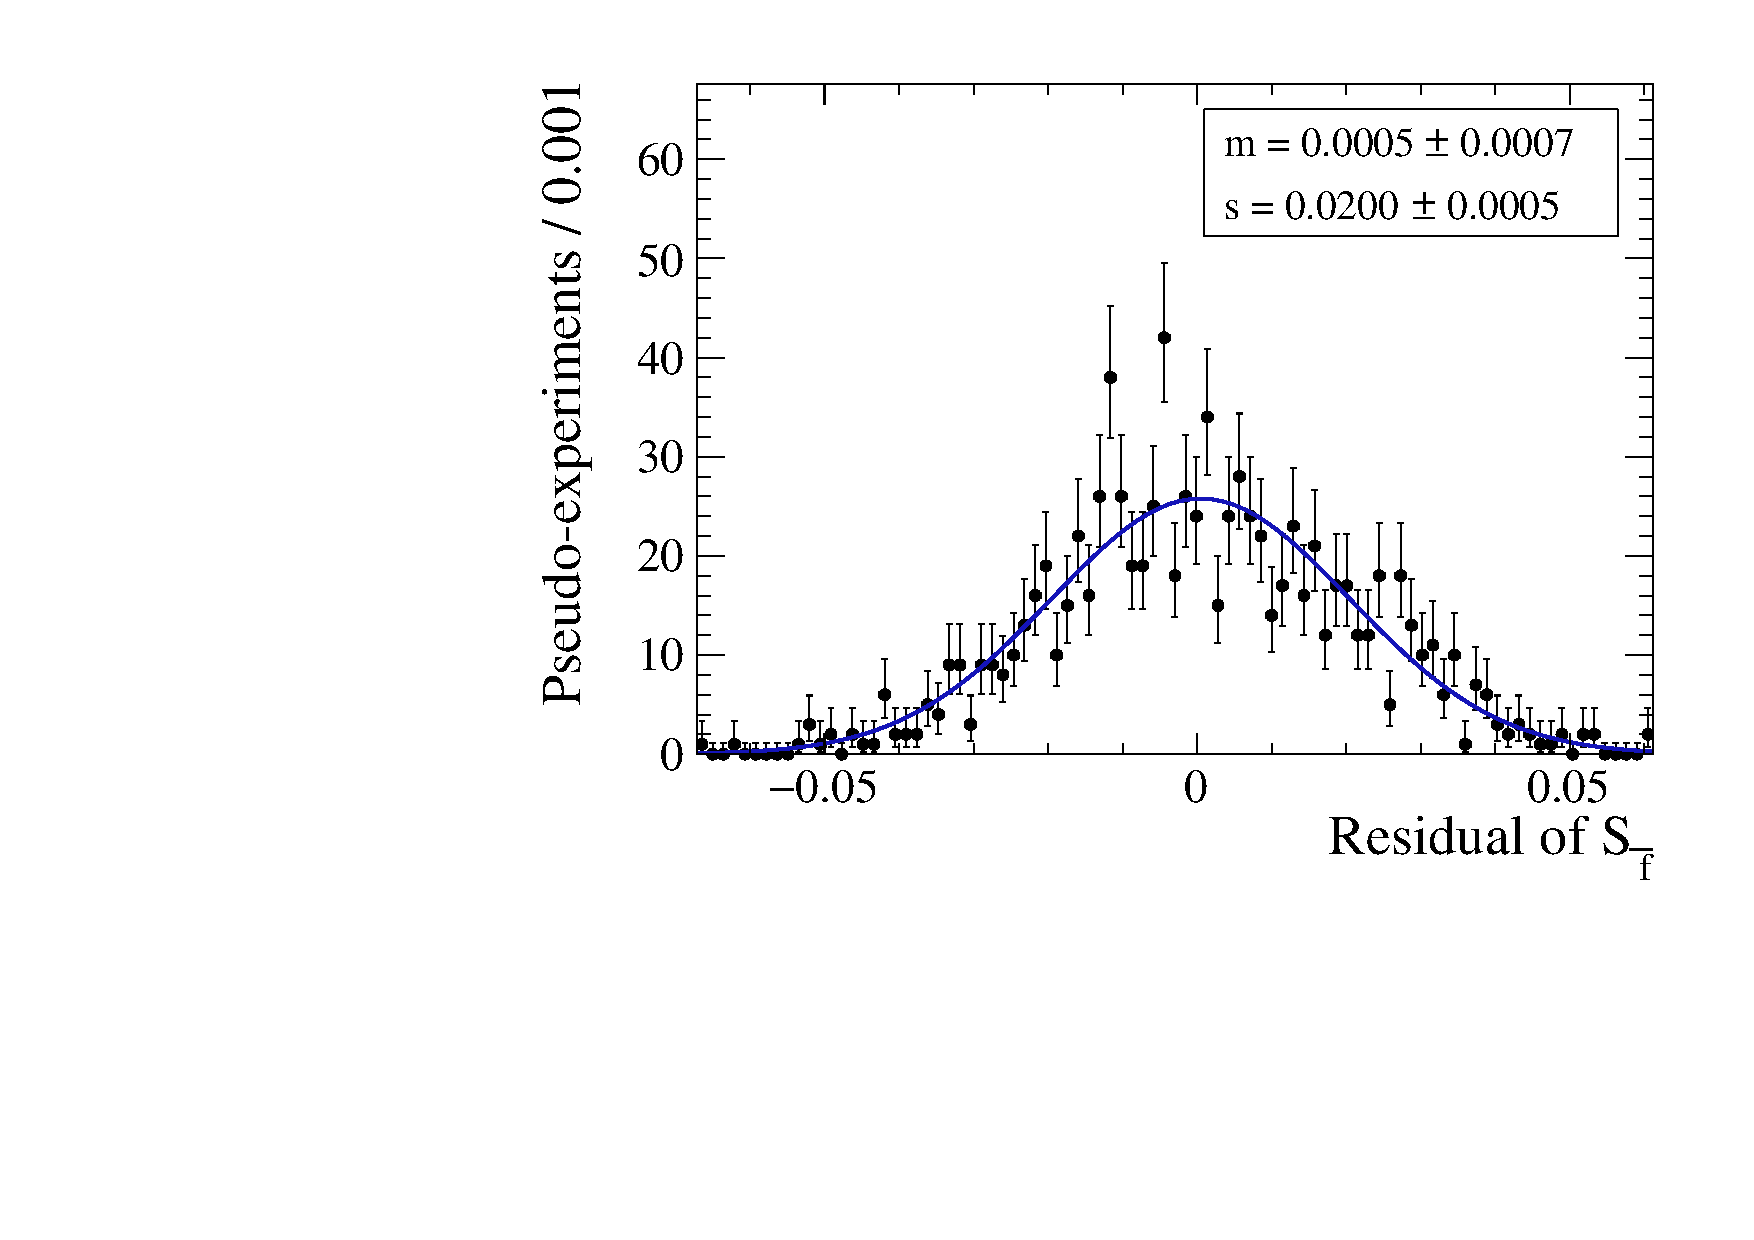
\includegraphics[width=0.4\textwidth]{06Systematics/figs/DG_Sfbar_res.pdf}
	\end{center}
        \vspace{-2mm}
	\caption{Distribution of $S_f$ (left) and $S_{\bar f}$ (right) residuals for the determination of the systematic uncertainty due the assumption $\DG=0$.}
	\label{fig:DGSystToys}
\end{figure}
